\chapter{Work Done}\label{C:workdone}

There were three main goals before the preliminary report. Firstly, create a framework to trace test spectrum. Secondly, find suitable bench marks and lastly, implement several different analysis methods.

\section{Creating the Framework}

The first goal of the project was to create a framework to trace tests and allow for different analysis methods to be added and changed with ease. The first question that arose was, what was the best way to execute every test in an efficient manner where I was able to run it again with limited effort. Since AspectJ with load time weaving was determined to be the best method to trace, a build automation tool would be best suited. The two main choices were Ant and Maven. After doing research, Ant appeared to give more control over the execution of JUnit tests. A control it gave was the ability to create a one new java virtual machine (JVM) before the tests were executed which would be used solely for the test suite. Since I was using a static class to hold the trace data, I needed the data to be held in memory until all the tests had run, which meant the tests had to be run with the same JVM. But the JVM had to be recreated as AspectJ load-time weaving requires its own class loader to be used through the command line java option.

The ability to allow for user defined pipeline is important in ensuring I don't have to hard code it. Ant uses it’s own JUnit runner class to execute the tests. This means that I am not able to input parameters into my project without executing the ant file through another main method and create the service that way. Doing this would be create messy and unwanted code. Therefore I decided to use a properties file, which would be loaded in during the static method construction. The purpose of this properties file was to not only allow me to change the setting of the run, such as the results file name, the type of service it should use but also allowing for a ‘pipeline’ approach to be used. This pipeline will be used for the analysis where the pipeline can specify the type of analysis and its setting, shown in figure 1.

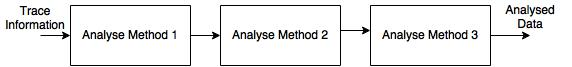
\includegraphics[width=\textwidth]{Pipeline.jpg}

\section{Finding Benchmarks}

The second goal was to find suitable benchmarks; this was harder it seemed. The benchmarks had to meet a criteria where they were java based, had large number of test cases (100 +) and were open source. Although there were 10 + benchmarks, the ability to use them depended on their build process. If they used maven, it was difficult to create a jar that contained the tests and often meant that I was not able to use the project as a benchmark. This eliminated several potential benchmarks and left the ant and gradle built projects. 

The current set of benchmarks is as following:

\begin{itemize}
\item Whiley
\item Java Compiler Kit
\item Jasm
\item Spring - Core
\item Metric-x - Core
\item Ant
\end{itemize}


Using ant as a benchmark created an unique situation. Since ant is used to run the JUnit tests, I have made my aspect ignore ant calls so that when ant is executing the tests it does not get traced. However, if I ignore Ant calls then the Ant benchmark can not be traced. This meant that I had to not use Ant to run itself but manually execute it. This was deemed worth the effort due to Ant’s current stature within the development community. 

\section{Implementing Analysis Methods}

The third goal was to use this data to analyse and determine the tests that are closely related. The first analysis stage that I decided to use was Levenshtein distance metric. This metric is the minimum number of single-character edits, in our case method calls, including insertions, deletions or substitutions. This method created some challenges. Firstly, the time to compare every test with every test becomes exponential. So as the analysis became more computationally heavy, the time to analysis the data increased. Secondly, due to there being thousands of tests and each test containing tens of thousands of method calls, memory management became crucial. 

My first approach was to resolve both issues by using a bloom filter approach. A bloom filter is a test where you determine whether an element is a member of a set or not, returning either "possibly in set" or "definitely not in set". In this case, it was used to determine whether the set of method calls for two tests were similar or not. The similarity and analysis type was set during within the property file. Looking at the set of method calls, rather than a list meant the number decreased from \todo{real example}. This approach was used under the hypothesis that the following is true.

$A, B, C, D \neq A, D, E, F, G$

$A, B, C, D \approx A, B, C, D, E$

That the first case the two tests would be not be redundant test’s due to having a high difference in method calls. However, there is a chance that the second test may be the same so it implies more computational heavy analysis should be done on it, such as using a list of method calls. This means that when using a list of method calls, the number of lists held in memory will be reduced as the number of tests will be decreased from the initial stage.

Although this made the analysing stage faster, it did not have any effect on the testing time. Each time that an analysis was to be run, the tests needed to be run at the same time. The approach used to get around this was to save the test data to disk. Such that the properties file can be set to save the data to disk, and when the data wants to be used without analysis, a main method is called. By using a regression analysis technique based on genetic algorithms, the original approach would correlate to the function:  

$6.0 + ((7.0 * (5.0 * ((X - 4.0) - (5.0 * 8.0)))) + (X * (X - 9.0)))$

Where X is the number of tests. So to complete the testing and analysis for 1300 tests, it would roughly take 1469666 seconds which is equal to 408.241 hours, or 17 days. However, analysing was still taking \todo{??}. To increase the performance of analysis, I decided to implement a concurrent method. From how I had implemented the framework this was able to be done with ease. At first there was an issue where the running it was on test situation, the results between concurrent and non concurrent was giving me the same result. However, on a benchmark the result was different. This required me to think about my how I was ensuring that the framework with the analysis. The test environment was too limited and David Pearce suggested that I create a larger test environment. Through doing this it allowed me to figure out where the errors were with the concurrent execution. \todo{increasing time by ?}

The next analysis implementation was the total difference. This method discarded the order of the methods for a test. Instead sorted them alphabetically and for every difference between the pairs, it added the 1 to the difference. This worked well in conjunction with the bloom filter approach, as it was a fast analysis pipeline. 

The next idea implemented was to take into account for the ‘calling context tree’. This means that for each method call, the graph contains a separate node for each call stack that the method can was called with  \todo{ref.}. What this involves in java terms is using the stack trace of the method and storing the depth specified within the properties file. This means that it is more difficult for a test to be similar to another as the calling tree of a method call is used.

The example that will be shown will be using the Whiley benchmark. From looking at the graphical representation \todo{in figure ?}, it shows the tests that are matching for Byte\_Valid\_5 test.

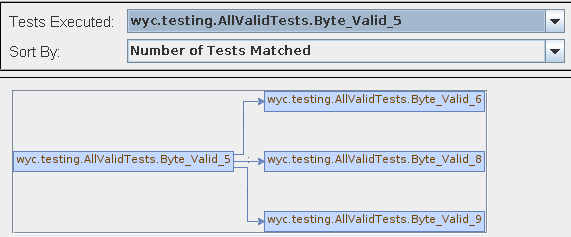
\includegraphics[width=\textwidth]{model24.png}

This requires us to conduct further examination of the test and as such the tests are from the Whiley Compiler tests, so looking at the Whiley files would give us insight into how closely related these two tests are. Comparing Byte\_Valid\_5 and Byte\_Valid\_8.

\textbf{Byte\_Valid\_8} \todo{Change these to code rather than images}
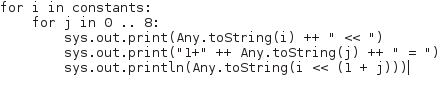
\includegraphics[]{model25.png}

\textbf{Byte\_Valid\_5}
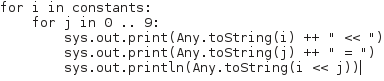
\includegraphics[]{model26.png}

This shows that the difference between the tests is the range of j and two additional addition statements. The decision whether these two tests are redundant is up to a developer. \todo{more?}


